\documentclass{beamer}
\usepackage[utf8]{inputenc}

\usetheme{Madrid}
\usecolortheme{default}
\usepackage{txfonts}
\usepackage{listings}
\usepackage{adjustbox}
\usepackage{tabularx}
\usepackage{lmodern}
\usepackage{circuitikz}
\usepackage{tikz}

\usepackage{gvv}
\usepackage{cite}
\usepackage{amsmath,amssymb,amsfonts,amsthm}
\usepackage{algorithmic}
\usepackage{graphicx}
\usepackage{textcomp}
\usepackage{xcolor}
\usepackage{txfonts}
\usepackage{listings}
\usepackage{enumitem}
\usepackage{mathtools}
\usepackage{gensymb}
\usepackage{comment}
\usepackage{tkz-euclide} 
\usepackage{listings}                                      
\def\inputGnumericTable{}                                
\usepackage{color}                                            
\usepackage{array}                                            
\usepackage{longtable}
\usepackage{multicol}
\usepackage{calc}                                             
\usepackage{multirow}                                         
\usepackage{hhline}                                           
\usepackage{ifthen}

\setbeamertemplate{page number in head/foot}[totalframenumber]

\usepackage{tcolorbox}
\tcbuselibrary{minted,breakable,xparse,skins}



\definecolor{bg}{gray}{0.95}
\DeclareTCBListing{mintedbox}{O{}m!O{}}{%
  breakable=true,
  listing engine=minted,
  listing only,
  minted language=#2,
  minted style=default,
  minted options={%
    linenos,
    gobble=0,
    breaklines=true,
    breakafter=,,
    fontsize=\small,
    numbersep=8pt,
    #1},
  boxsep=0pt,
  left skip=0pt,
  right skip=0pt,
  left=25pt,
  right=0pt,
  top=3pt,
  bottom=3pt,
  arc=5pt,
  leftrule=0pt,
  rightrule=0pt,
  bottomrule=2pt,
  toprule=2pt,
  colback=bg,
  colframe=orange!70,
  enhanced,
  overlay={
    \begin{tcbclipinterior}
    \fill[orange!20!white] (frame.south west) rectangle ([xshift=20pt]frame.north west);
    \end{tcbclipinterior}},
  #3,
}
\lstset{
    language=C,
    basicstyle=\ttfamily\small,
    keywordstyle=\color{blue},
    stringstyle=\color{orange},
    commentstyle=\color{green!60!black},
    numbers=left,
    numberstyle=\tiny\color{gray},
    breaklines=true,
    showstringspaces=false,
}

\title 
{4.3.20}
\date{September 29, 2025}


\author 
{Sai Sreevallabh - EE25BTECH11031}



\begin{document}


\frame{\titlepage}
\begin{frame}{Question}
Find the ratio in which the Y-axis divides the line segment joining the points $\brak{5,-6}$ and $\brak{-1,-4}$. Also find the point of intersection. \\
\end{frame}



\begin{frame}{Theoretical Solution}

Given points are\\
\begin{align}
    \vec{A}=\myvec{5\\-6} \ \text{and}\  \vec{B}=\myvec{-1\\-4}
\end{align}

Let $\vec{P}$ be a point on the Y-axis. We can assume it to be

\begin{align}
    \vec{P}=\myvec{0\\y}
\end{align}

\end{frame}

\begin{frame}{Theoretical Solution}

$\vec{A}$, $\vec{B}$ and $\vec{P}$ are collinear. 

\begin{align}
    \vec{P}-\vec{A}=\myvec{-5 \\ y+6} \ , \ 
    \vec{B}-\vec{A}=\myvec{-6\\2}  
\end{align}

\begin{align}
    \myvec{\vec{P}-\vec{A} & \vec{B}-\vec{A}}^T =& \myvec{-5 & -6\\ y+6 & 2}^T\\
    =& \myvec{-5 & y+6 \\ -6 & 2}
\end{align}

\end{frame}

\begin{frame}{Theoretical Solution}
Converting into echelon form using row operations

\begin{align}
    \myvec{x-1 & -3 \\ 3 & 2}\ \xleftrightarrow[]{R_2 \to R_2-\frac{6}{5}R_1} \  \myvec{-5 & y+6 \\ 0 & \frac{-6y-26}{5}}
\end{align}

The points are collinear. Hence the rank of the above matrix must be 1. So, 

\begin{align}
    &\frac{6y+26}{5} = 0\\
    \implies& y=-\frac{13}{3}
\end{align}\\

\end{frame}

\begin{frame}{Theoretical Solution}
Let $\vec{P}$ divide the line joining points $\vec{A}$ and $\vec{B}$ in the ratio $k:1$. 

\begin{align}
    \vec{P}=\frac{k\vec{B}+\vec{A}}{k+1}
\end{align}

\begin{align}
    k\brak{\vec{P}- \vec{B}} = \vec{A}-\vec{P}
\end{align}

\begin{align}
    k=\frac{\brak{\vec{P}-\vec{B}}^T\brak{\vec{A}-\vec{P}}}{||\brak{\vec{P}-\vec{B}}||^2}
\end{align}
\end{frame}

\begin{frame}{Theoretical Solution}
    \begin{align}
      k=\frac{\myvec{1 & y+4}\myvec{5\\-y-6}}{{\norm{\myvec{1 \\ y+4}}}^2}
\end{align}

Substituting the value of $y$ as $-\frac{13}{3}$, we get the value of k as

\begin{align}
    k=5
\end{align}

$\therefore$ The point $\vec{P}\myvec{0\\-\frac{13}{3}}$ on the X-axis divides the line segment in the ratio $5:1$. 
\end{frame}


\begin{frame}[fragile]
    \frametitle{C Code - Function to Find y Coordinate of P}

    \begin{lstlisting}

#include <stdio.h>
#include <math.h>

double Solve_for_y(double A[2], double B[2]){
	
	double k = -A[0]/B[0];
	double y = (A[1]+(k*B[1]))/(k+1);

	return y;
}
    \end{lstlisting}

\end{frame}

\begin{frame}[fragile]
    \frametitle{Python Code - Using Shared Object}
    \begin{lstlisting}
import numpy as np
import numpy.linalg as LA
import matplotlib.pyplot as plt
import ctypes

c_lib=ctypes.CDLL('./code.so')

c_lib.Solve_for_y.argtypes = [
        ctypes.c_double*2,
        ctypes.c_double*2
        ]

c_lib.Solve_for_y.restype = ctypes.c_double

A = (ctypes.c_double*2)(5.0, -6.0) 
B = (ctypes.c_double*2)(-1.0, -4.0)

\end{lstlisting}
\end{frame}

\begin{frame}[fragile]
    \frametitle{Python Code - Using Shared Object}
    \begin{lstlisting}

y = c_lib.Solve_for_y(A,B)

y = np.round(y,2)

A = np.array([5,-6]).reshape(-1,1) 
B = np.array([-1,-4]).reshape(-1,1)

P = np.array([0.0,y]).reshape(-1,1)

plt.plot([A[0,0], B[0,0]], [A[1,0], B[1,0]], label="Line Segment $AB$")

x = np.array([A[0,0], B[0,0], P[0,0]])
y = np.array([A[1,0], B[1,0], P[1,0]])

\end{lstlisting}
\end{frame}

\begin{frame}[fragile]
    \frametitle{Python Code - Using Shared Object}
    \begin{lstlisting}
    
plt.scatter(x,y, c='red')

vert_labels = ['A', 'B', 'P']

for i,txt in enumerate(vert_labels):
    plt.annotate(f'{txt}\n({x[i]},{y[i]})',
                  (x[i],y[i]),
                  textcoords = "offset points",
                  xytext = (20,5),
                  ha = 'center')

\end{lstlisting}
\end{frame}



\begin{frame}[fragile]
    \frametitle{Python Code - Using Shared Object}
    \begin{lstlisting}
    
ax = plt.gca()
ax.spines['top'].set_color('none')
ax.spines['left'].set_position('zero')
ax.spines['right'].set_color('none')
ax.spines['bottom'].set_position('zero')
plt.xlabel('$x$')
plt.ylabel('$y$')
plt.legend(loc='best')
plt.grid() 
plt.axis('equal')

plt.savefig("../Figs/plot(py+C).png")

plt.show()

\end{lstlisting}
\end{frame}

\begin{frame}{Plot-Using Both C and Python}
    \centering
    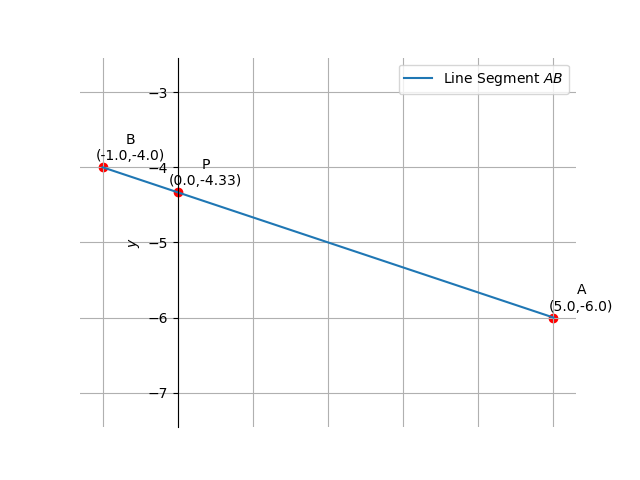
\includegraphics[width=\columnwidth, height=0.8\textheight, keepaspectratio]{Figs/plot(py+C).png}     
\end{frame}

%-------End of Python+C-------------


\begin{frame}[fragile]
    \frametitle{Python Code}
    \begin{lstlisting}
import math
import numpy as np
import matplotlib.pyplot as plt
import numpy.linalg as LA

A = np.array([5,-6])
B = np.array([-1,-4])

k = -(A[0])/(B[0])

y = (A[1] + k*B[1])/(k+1)

y = np.round(y,2)

\end{lstlisting}
\end{frame}

\begin{frame}[fragile]
    \frametitle{Python Code}
    \begin{lstlisting}

P = np.array([0.0,y]).reshape(-1,1)

A = A.reshape(-1,1)
B = B.reshape(-1,1)

plt.plot([A[0,0], B[0,0]], [A[1,0],B[1,0]], label = "Line Segment $AB$")

x = np.array([A[0,0], B[0,0], P[0,0]])
y = np.array([A[1,0], B[1,0], P[1,0]])

plt.scatter(x,y, c='red')



\end{lstlisting}
\end{frame}

\begin{frame}[fragile]
    \frametitle{Python Code}
    \begin{lstlisting}

vert_labels = ['A', 'B', 'P']

for i,txt in enumerate(vert_labels):
    plt.annotate(f'{txt}({x[i]},{y[i]})',
                  (x[i],y[i]),
                  textcoords = "offset points",
                  xytext = (20,5),
                  ha = 'center')
\end{lstlisting}
\end{frame}

\begin{frame}[fragile]
    \frametitle{Python Code}
    \begin{lstlisting}
ax = plt.gca()
ax.spines['top'].set_color('none')
ax.spines['bottom'].set_position('zero')
ax.spines['right'].set_color('none')
ax.spines['left'].set_position('zero')
plt.xlabel('x')
plt.ylabel('y')
plt.legend(loc='best')
plt.grid()
plt.axis('equal')

plt.savefig("../Figs/plot(py).png")
plt.show()



    \end{lstlisting}
\end{frame}


\begin{frame}{Plot-Using Python only}
    \centering
    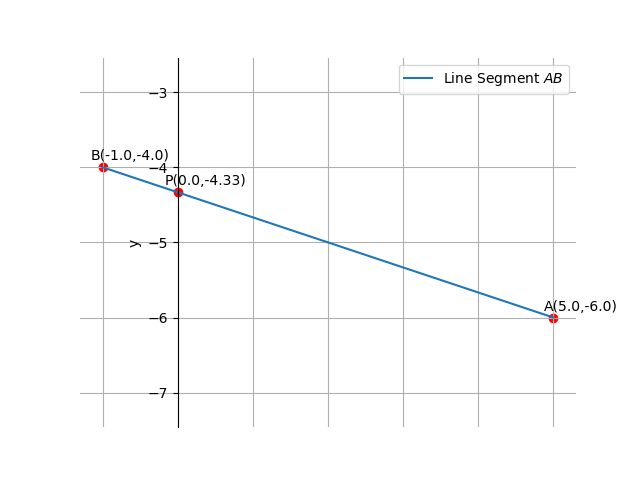
\includegraphics[width=\columnwidth, height=0.8\textheight, keepaspectratio]{Figs/plot(py).png}     
\end{frame}


\end{document}
